
\documentclass[hide notes,intlimits]{beamer}


\mode<presentation>
{
  \usetheme[headline,footline]{UAFshade}
  \setbeamercovered{transparent}
}

% load packages
\usepackage[english]{babel}
\usepackage[latin1]{inputenc}
\usepackage[T1]{fontenc}
\usepackage{multimedia,pgf}
\usepackage{lmodern}
\usepackage[amssymb]{SIunits}
\usepackage{hyperref}
\usepackage{natbib}
\bibliographystyle{andy}


% title page
\title[Glacier Dynamics] % (optional, use only with long paper titles)
{Mechanics and Thermodynamics of Glaciers}
\subtitle{Glaciers 617}


\author[Aschwanden] % (optional, use only with lots of authors)
{Andy Aschwanden}
% - Give the names in the same order as the appear in the paper.
% - Use the \inst{?} command only if the authors have different
%   affiliation.

\institute[ARSC] % (optional, but mostly needed)
{
  %
  Arctic Region Supercomputing Center\\
  University of Alaska Fairbanks, USA
}
% - Use the \inst command only if there are several affiliations.
% - Keep it simple, no one is interested in your street address.




\subject{Glaciers}

% define what is shown at the beginning of each section
\AtBeginSection[]
{
 \begin{frame}<beamer>
   \frametitle{Outline}
   \tableofcontents[currentsection,subsectionstyle=hide/show/hide]
 \end{frame}
}

% define what is shown at the beginning of each subsection
\AtBeginSubsection[]
{
 \begin{frame}<beamer>
  \frametitle{Outline}
   \tableofcontents[currentsection,currentsubsection]
 \end{frame}
}

\begin{document}

% insert titlepage
\begin{frame}
  \titlepage
\end{frame}

% insert TOC
\begin{frame}
 \frametitle{Outline}
 \tableofcontents[subsectionstyle=hide]
  %You might wish to add the option [pausesections]
\end{frame}

\section{Introduction}


%{
%\setbeamertemplate{headline}[default]
%\begin{frame}
%  \frametitle{Why}
%  The flow of glaciers and ice sheets is an interesting, non-trival problem in fluid dynamics
%\end{frame}
%} 

\plainframe{
  \begin{figure}
    \pgfputat{\pgfxy(-.39,.25)}{
    \includegraphics<1>[width=\paperwidth]{figures/gorner}%
    \includegraphics<2>[width=\paperwidth]{figures/gorner_clarke}%    
  }
  \end{figure}
}

\begin{frame}
  \frametitle{Course Material}
  \begin{itemize}
    \item notation follows closely \cite{GreveBlatter_disg}
    \item covers Chapter~3\,--\,5.1
    \item \url{http://www.gi.alaska.edu/~aaschwanden/lecture.html}
  \end{itemize}
  \def\newblock{}
  \bibliography{cryo}
\end{frame}


\begin{frame}
  \frametitle{Observations}
  \centering{
    \includegraphics<1>[width=\textwidth]{figures/agassi}%
  }
\end{frame}

\begin{frame}
  \frametitle{Observations}
  \begin{columns}
    \column[C]{4.25cm}
    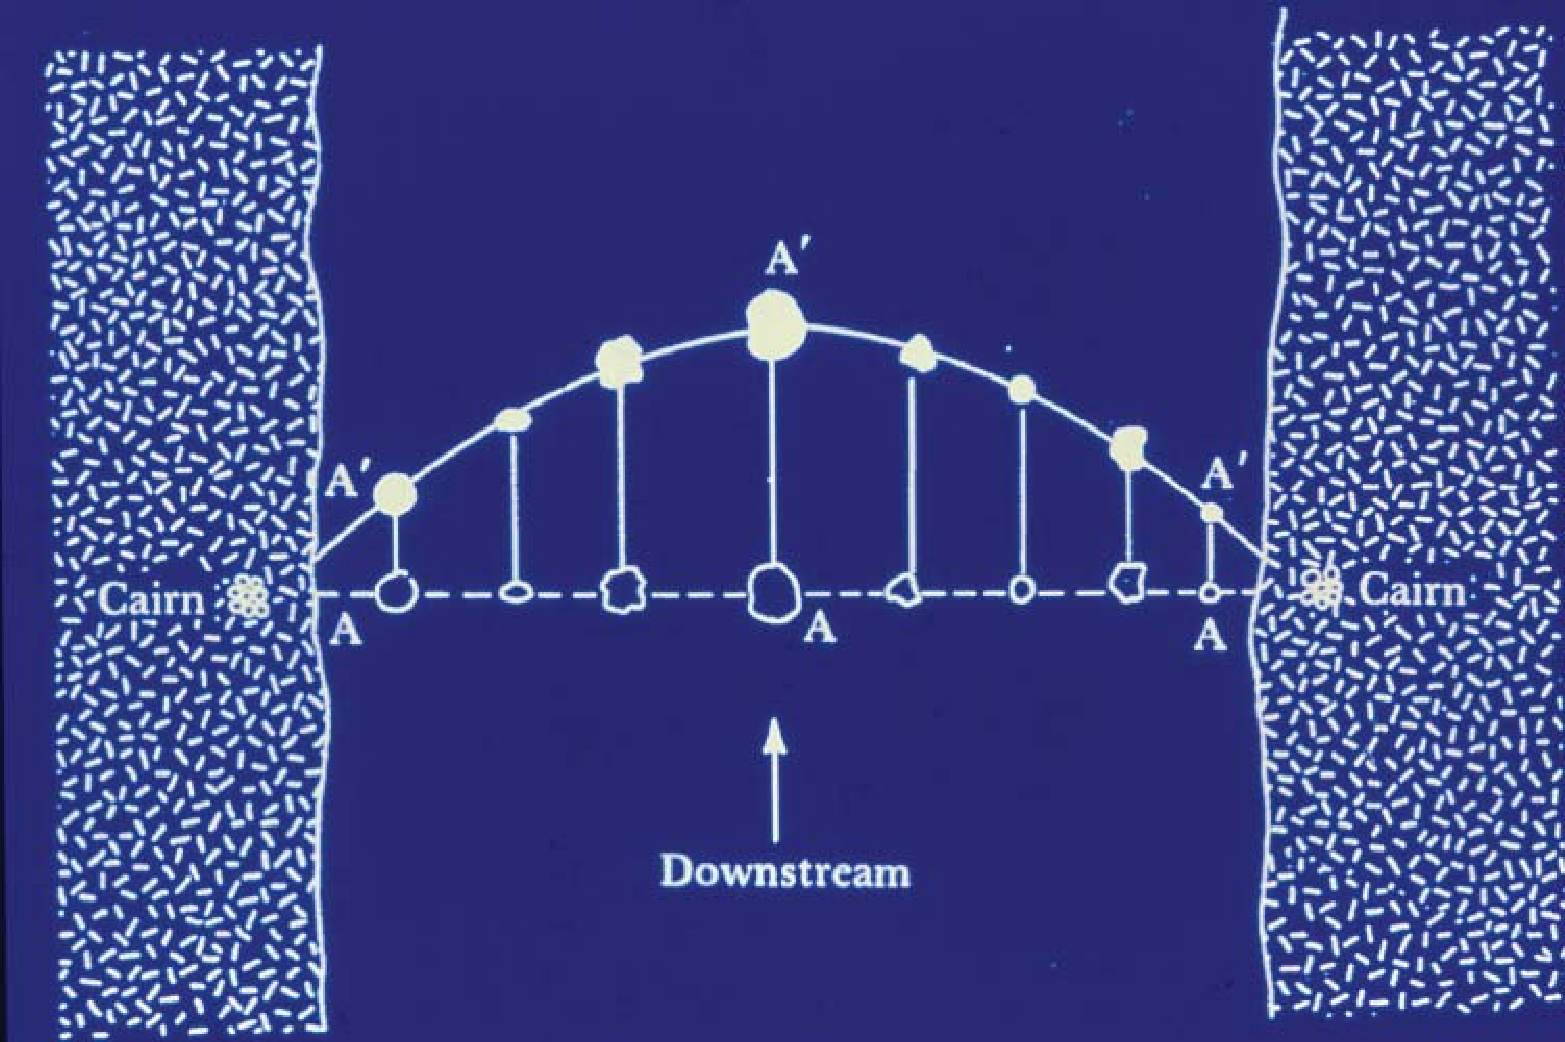
\includegraphics[width=4cm]{figures/geschw_prof_oberfl}%
    \vskip1em
    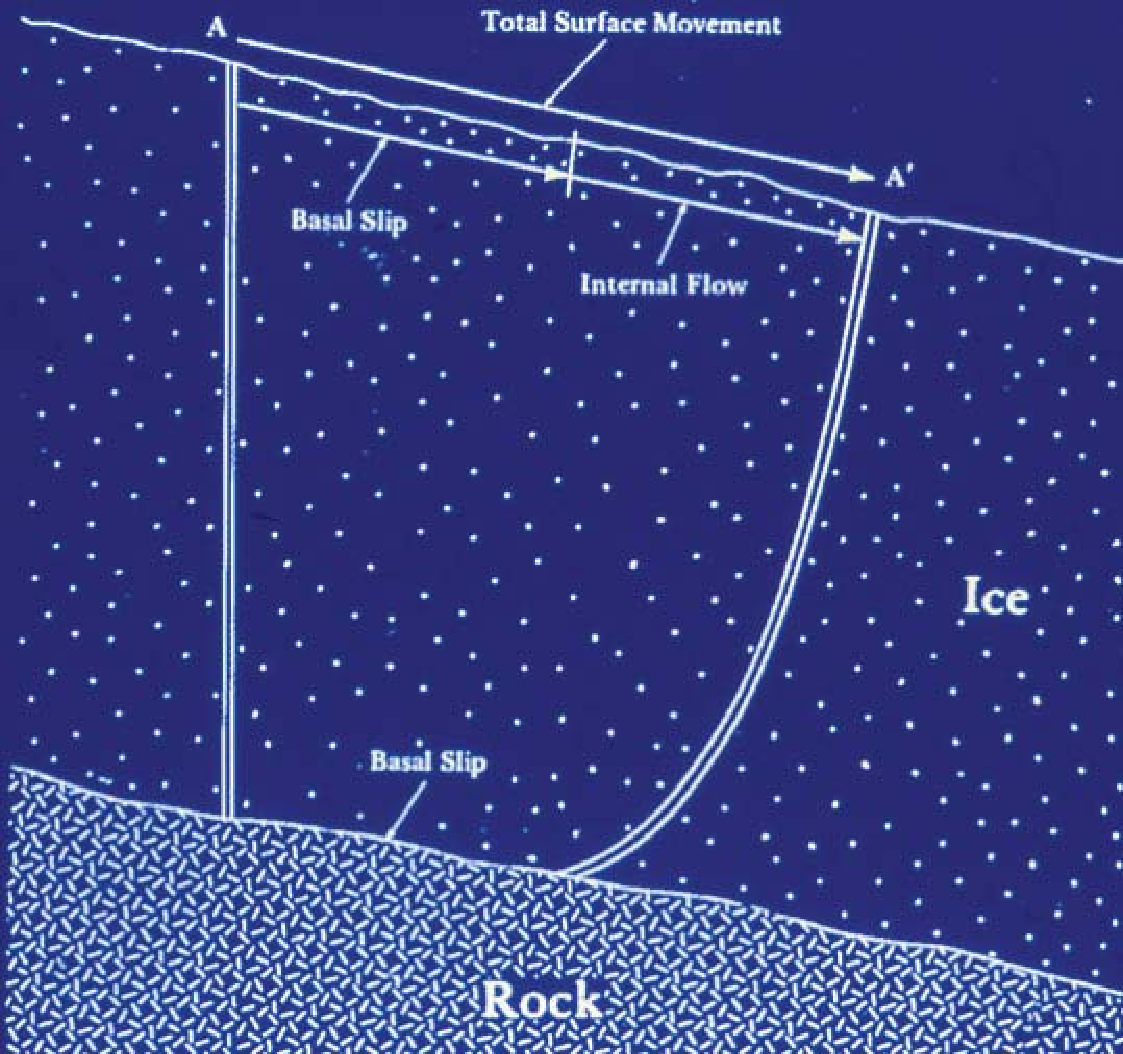
\includegraphics[width=4cm]{figures/geschw_vert_prof}%
    \column[C]{7.75cm}
    \begin{block}{1779 Gravitation theory by de~Saussure}
      H.~B. de~Saussure observes sliding: 
      \begin{itemize}
        \item ``\ldots the weight of the ice might be sufficient to urge it down the slope of the valley, if the sliding motion were aided by the water flowing at the bottom.''
      \end{itemize}
    \end{block}
 \end{columns}
\end{frame}


\begin{frame}
  \frametitle{Observations}
  \begin{columns}
    \column[C]{4.25cm}
    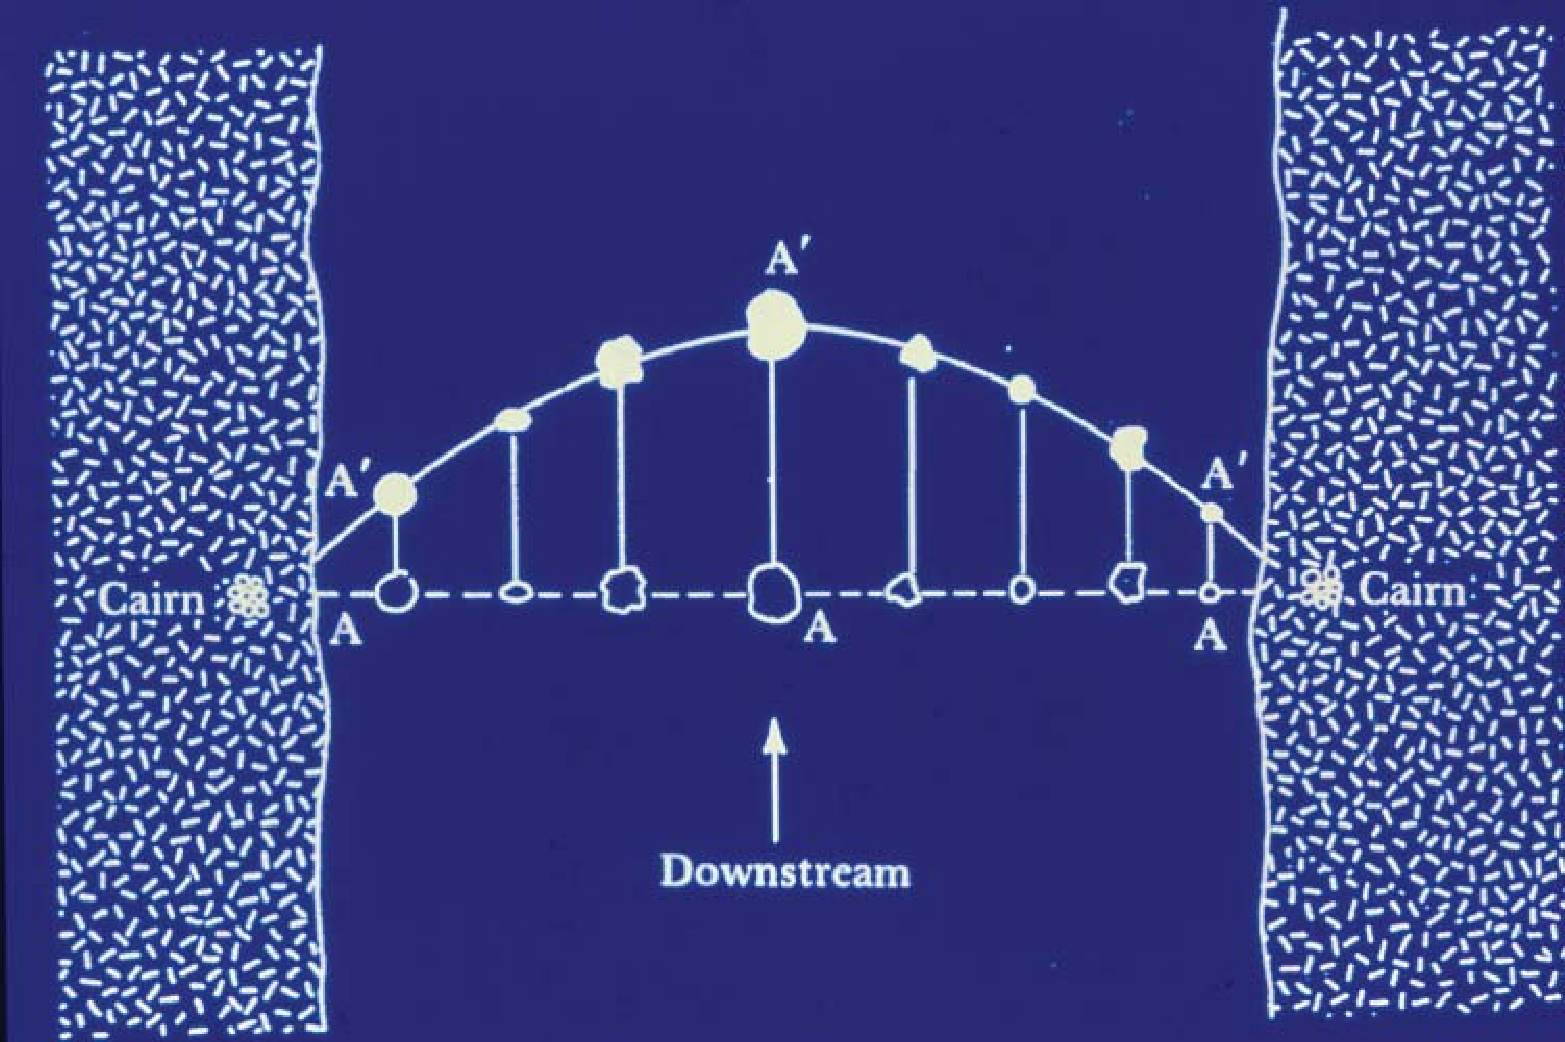
\includegraphics[width=4cm]{figures/geschw_prof_oberfl}%
    \vskip1em
    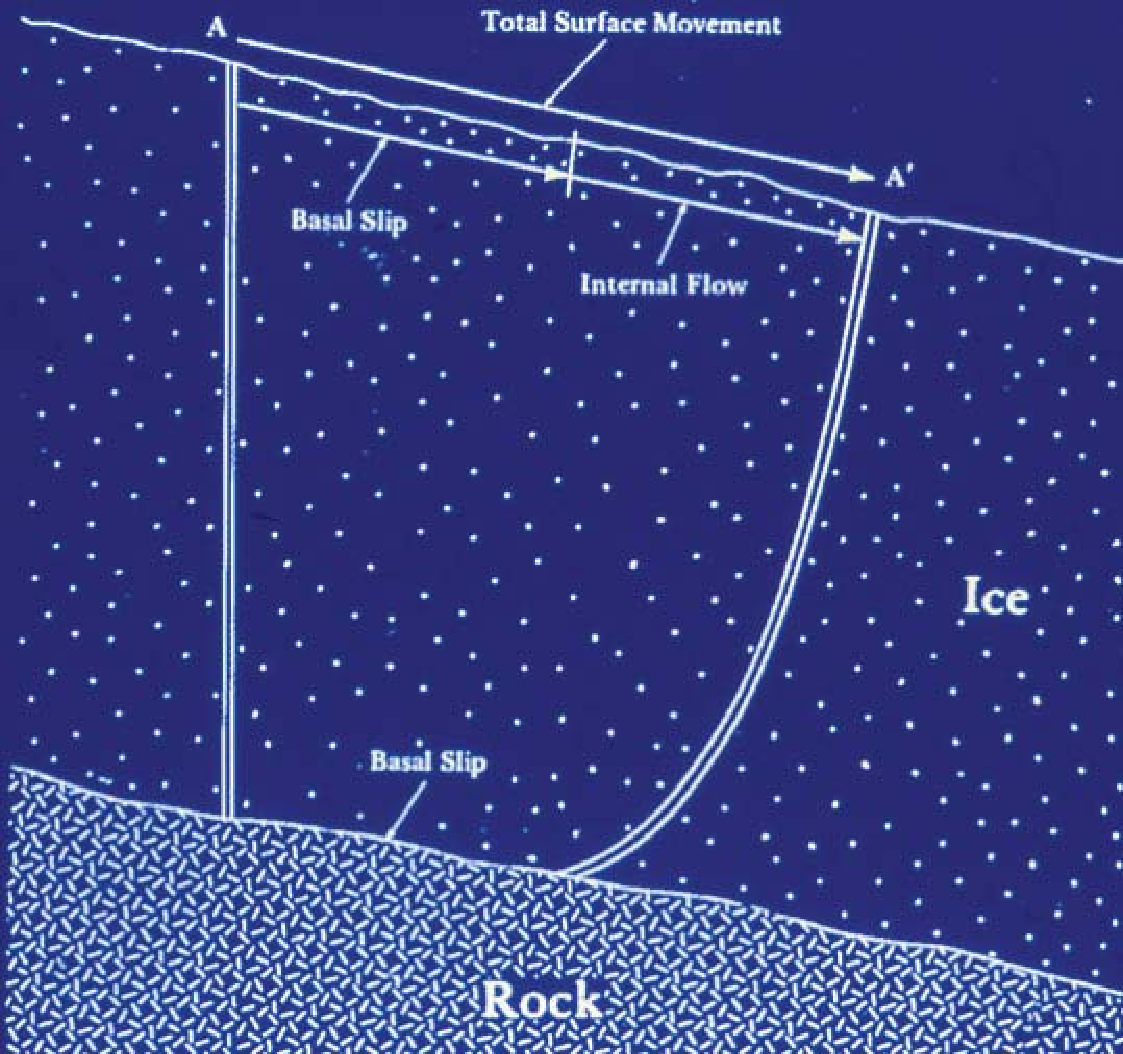
\includegraphics[width=4cm]{figures/geschw_vert_prof}%
    \column[C]{7.75cm}
    \begin{block}{1840-1846 Dilatation theory by L. Agassi}
      \begin{itemize}
        \item glacier ice contains innumerable fissures and capillary tubes
        \item during the day, these tubes imbibe the water
        \item and during the night, the water freezes
        \item this distension exertcs a force and propels the glacier in the direction of least resistance
      \end{itemize}
    \end{block}
 \end{columns}
\end{frame}


\begin{frame}
  \frametitle{Observations}
  \begin{columns}
    \column[C]{4.25cm}
    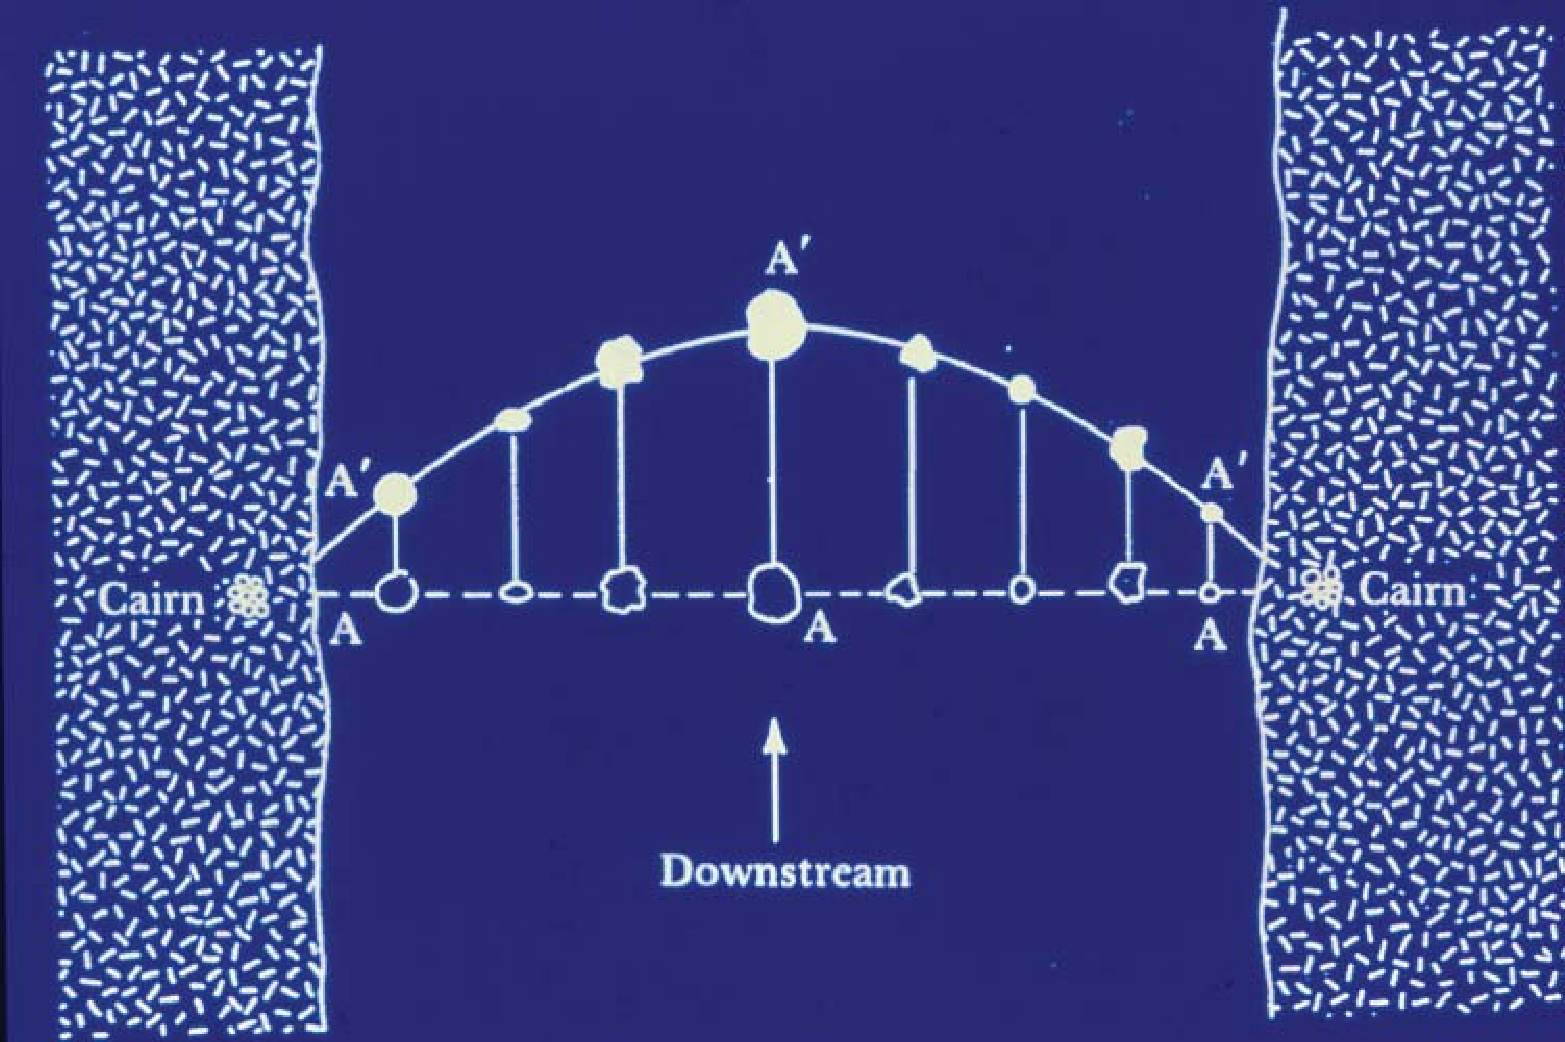
\includegraphics[width=4cm]{figures/geschw_prof_oberfl}%
    \vskip1em
    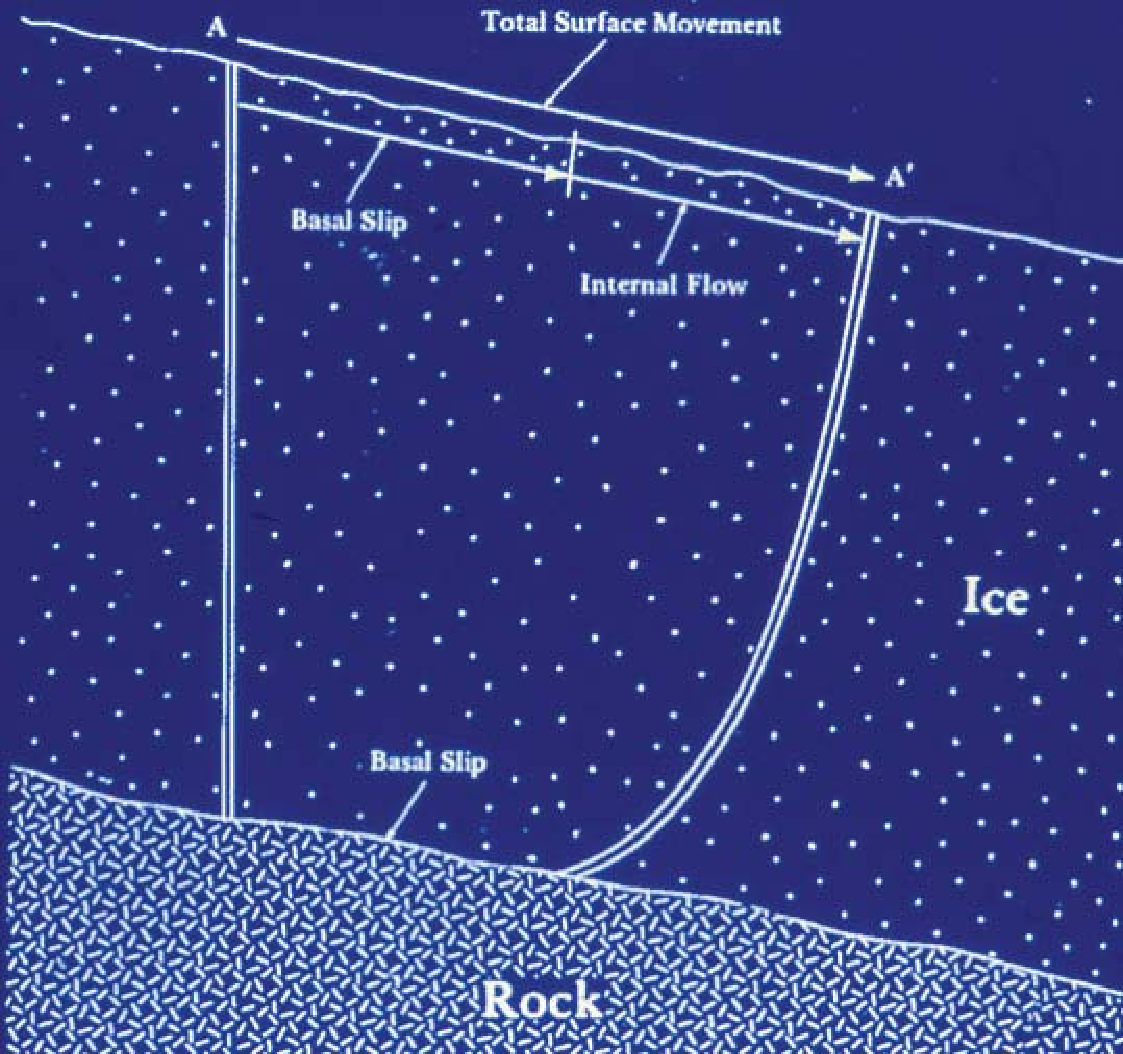
\includegraphics[width=4cm]{figures/geschw_vert_prof}%
    \column[C]{7.75cm}
    \begin{block}{1864-1930 Viscous flow theory by J.~Forbes}
      \begin{itemize}
        \item made his own observations on Mer de Glace, France
          \item glacier flows fastest in the center
        \item opposes Agassi' theory, if the dilatation theory were true
        \item then flow would be greatest at sunset
        \item and near the glacier margins
      \end{itemize}
    \end{block}
 \end{columns}
\end{frame}

 
\begin{frame}
  \frametitle{Questions}
  \centering{
    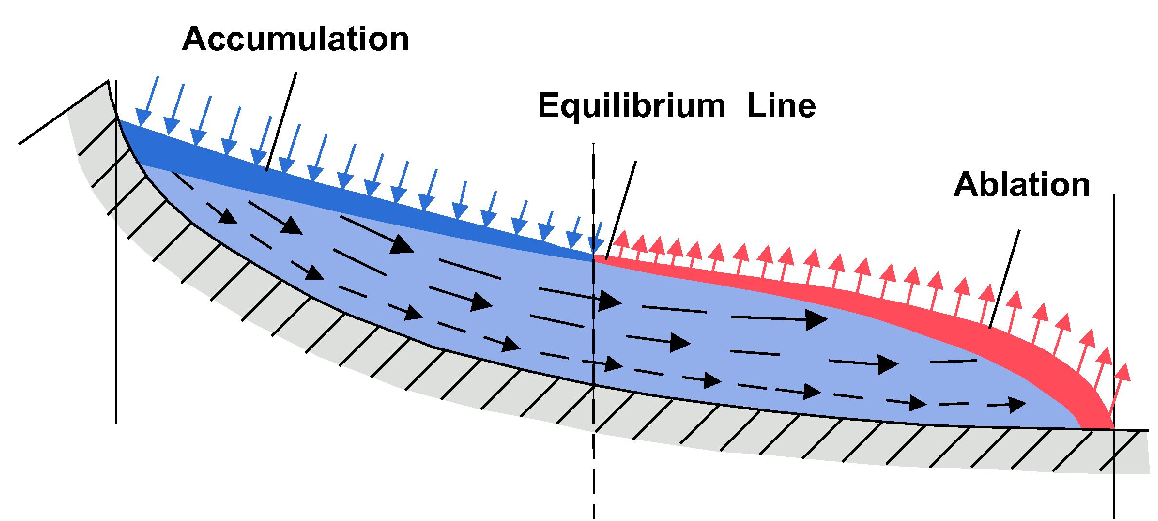
\includegraphics[width=.65\textwidth]{figures/flow_acc_abl}
  }
 \begin{itemize}
    \item What determines the glacier shape and extend
    \item How do ablation, accumulation, ice temperature, and the bedrock topography influence the flow of a glacier
    \item How does the flow speed vary with depth, along a flowline, or orthogonal to a flowline
  \end{itemize}
\end{frame}

\begin{frame}
  \frametitle{Questions}
  \centering{
    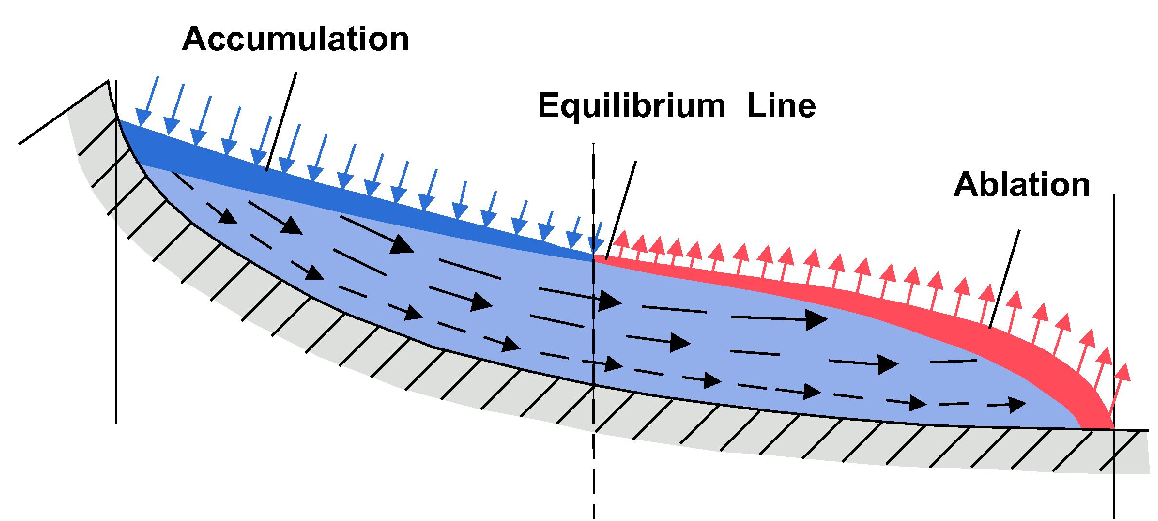
\includegraphics[width=.5\textwidth]{figures/flow_acc_abl}
  }
 \begin{block}{The two major problems}
   \begin{enumerate}
   \item Given the boundary conditions,
     \begin{itemize}
     \item basal topography
     \item accumulation-ablation function
     \item temperature at the upper ice surface
     \item geothermal heat flux at the base,
   \end{itemize}
   which glacier (geometry) is in equilibrium for given bc's.
  \item How does the glacier respond to changes in the bc's?
\end{enumerate}
  \end{block}
\end{frame}

\begin{frame}
  \frametitle{Answer}
  \centering{
    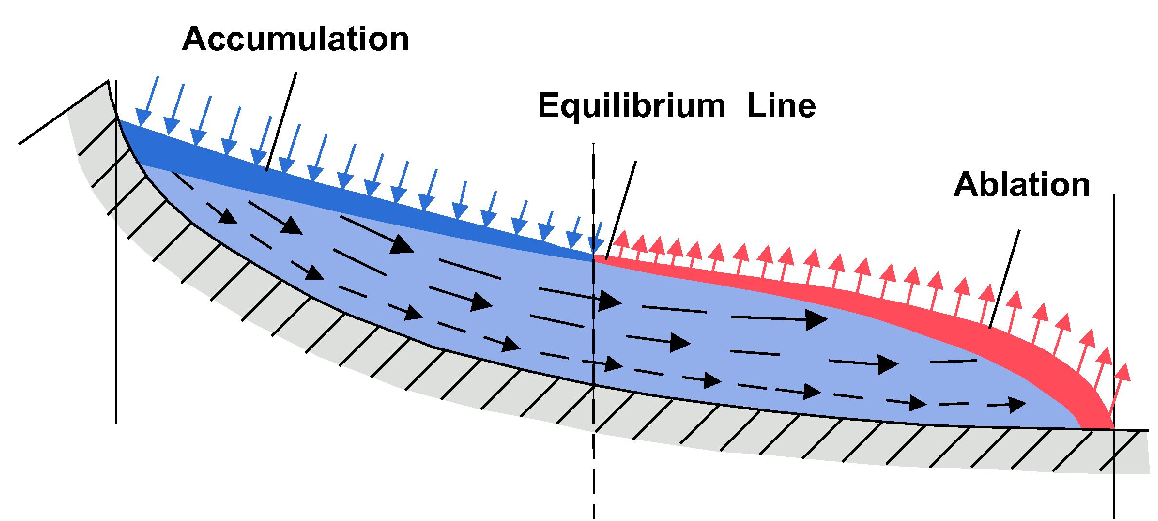
\includegraphics[width=.5\textwidth]{figures/flow_acc_abl}
  }

 \begin{block}{Solution: Continuums Mechanics \& Rheology}
   \begin{itemize}
     \item Solve balance equations for
       \begin{itemize}
       \item mass
       \item linear and angular momentum
       \item energy
       \item (forget about entropy)
       \end{itemize}
     \item Define constitutive equations
  \end{itemize}
\end{block}
\end{frame}


\section{Balance Equations}

\begin{frame}
  \frametitle{General Balance Equations}
  \begin{equation*}
   \frac{\partial g}{\partial t} = - \nabla \cdot \left(\boldsymbol{\phi} + g\mathbf{v}\right) + p + s
 \end{equation*}
 \begin{columns}
   \column[C]{0.1cm}
   $g$ \\
   $\boldsymbol{\phi}$ \\
   $p$ \\
   $s$ \\
   \column[C]{6cm}
   physical quantity \\
   flux of $g$ through the boundary \\
   production of $g$ \\
   supply of $g$
 \end{columns}
\end{frame}


\begin{frame}
  \frametitle{Balance Equations}
  \large{
  \begin{equation*}
  \begin{array}{lcclc}
    \text{mass} \quad &  \frac{\text{d} \rho}{\text{d} t} & = & -\rho\nabla \cdot \mathbf{v} \quad & (1)\\[.25em]
    \text{momentum} \quad & \frac{\text{d} \mathbf{v}}{\text{d} t} & = & -\nabla \cdot \mathbf{T} - \mathbf{f} \quad & (3) \\[.25em]
    \text{internal energy} \quad & \frac{\text{d} u}{\text{d} t} & = & - \nabla \cdot \mathbf{q} + \text{tr} \left(\mathbf{T}\cdot\mathbf{D}\right) \quad & (1)
  \end{array}
  \end{equation*}
  }
\centering{
 \begin{columns}
   \column[T]{4cm} \centering{
   left-hand side \\
   $\rho$ (1)\\
   $\mathbf{v}$ (3)\\
   $u$ (1)
   }
   \column[T]{4cm} \centering{
   right-hand side \\
   $\mathbf{T}$ (6)\\
   $\mathbf{q}$ (3)
  }
 \end{columns}
  }
  \begin{itemize}
   \item so we have 5 equations for 14 unknown fields
   \item the system is highly under-determined
   \item[$\Rightarrow$] \alert{closure relations} required
 \end{itemize}
\end{frame}


\begin{frame}
  \frametitle{Closure Relations}
  \begin{itemize}
    \item \alert{balance equations} are universally valid
    \item \alert{closure relations} describe the specific behavior of a material
    \item \alert{closure relations} are often called \alert{constitutive equations}
  \end{itemize}
\end{frame}


\begin{frame}
  \frametitle{Balance Equations for Glaciers}
  \large{
  \begin{equation*}
  \begin{array}{lcclc}
    \text{mass} &  \nabla \cdot \mathbf{v} & = & 0 \quad & (3)\\
    \text{momentum} & \nabla \cdot \mathbf{T} & = & - \rho \mathbf{g} \quad & (3)\\
    \text{internal energy} & \frac{\text{d} u}{\text{d} t} & = & - \nabla \cdot \mathbf{q} + \text{tr}\left(\mathbf{T}\cdot\mathbf{D}\right) \quad & (1)
  \end{array}
  \end{equation*}
  }
\centering{
 \begin{columns}
   \column[T]{4cm} \centering{
   left-hand side \\
   $\mathbf{v}$ (3)\\
   $\mathbf{T}$ (6)\\
   $u$ (1)
   }
   \column[T]{4cm} \centering{
   right-hand side \\
  $\mathbf{q}$ (3)
  }
 \end{columns}
  }
  \begin{itemize}
   \item so we have 7 equations for 13 unknown fields
   \item the system is highly under-determined
   \item[$\Rightarrow$] \alert{closure relations} required
 \end{itemize}
\end{frame}


\section{Constitutive Equations}

\begin{frame}
  \frametitle{Constitutive Equations for Glaciers}
  \begin{itemize}
    \item for the heat flux $\mathbf{q}$
    \item for the viscosity $\eta$
  \end{itemize}
\end{frame}


\begin{frame}
  \frametitle{Constitutive Equations for Glaciers}
  \begin{itemize}
    \item ask a material scientist or rheologist
    \item and let him/her do some fancy experiments
 \end{itemize}
\end{frame}


\begin{frame}
  \frametitle{Constitutive Equations for Glaciers}
  From experiments, you will learn that ice behaves like a
  \begin{itemize}
    \item viscous
    \item non-Newtionian
    \item heat-conduction
 \end{itemize}
fluid. So what does this mean?
\end{frame}


\begin{frame}
  \frametitle{Constitutive Equations for Glaciers}
  \begin{block}{Viscous material}
 \begin{itemize}
    \item deformation rate $\propto$ stress
\end{itemize}
 \end{block}
  \begin{block}{Non-Newtonian fluid}
 \begin{itemize}
    \item non-linear relationship between deformation rate and stress
\end{itemize}
 \end{block}
\end{frame}


\section{Glaciers}


\subsection{Balance Equations}

\begin{frame}
  \frametitle{Large-Scale Dynamics}
  \begin{itemize}
    \item Ice sheets are glaciers too!
  \end{itemize}
  \vskip1em
  \centering{
    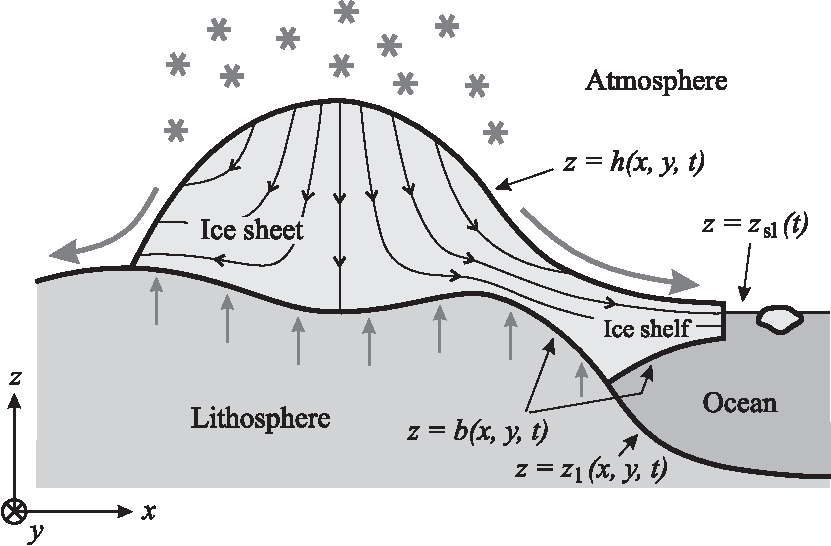
\includegraphics[width=.75\textwidth]{figures/fig_5_01}%
    }
\end{frame}

\begin{frame}
  \frametitle{Large-Scale Dynamics}
  \begin{block}{Some typical values for an ice sheet}
  \begin{equation*}
  \begin{array}{rccl}
    \text{horizontal extend} &  [L] & = & \unit{1000}\kilo\meter\\
    \text{vertical extend} & [H] & = & \unit{1}\kilo\meter \\
    \text{horizontal velocity} & [U] & = & \unit{100}\meter\power{a}{-1}\\
    \text{vertical velocity} & [W] & = & \unit{0.1}\meter\power{a}{-1}\\
    \text{pressure} & [U] & = & \rho g[H] = \unit{10}\mega\pascal\\
    \text{time-scale} & [T] & = &[L]/[U] = 10^{4}\usk\power{a}{1}\\
  \end{array}
  \end{equation*}
  \end{block}
  The aspect ratio $\epsilon$ is defined as
  \begin{equation*}
    \epsilon = \frac{[H]}{[L]} = \frac{[U]}{[W]} = 10^{-3} \text{ for an ice sheet}
  \end{equation*}
  \begin{itemize}
    \item The scaling argument for valley glaciers is almost the same
   \end{itemize}
\end{frame}


\begin{frame}
  \frametitle{Large-Scale Dynamics}
  \begin{block}{Froude number}
    The \alert{Froude number $Fr$} is the ratio of acceleration and pressure gradient. In the horizontal we have
  \begin{equation*}
    Fr = \frac{\rho[U]/[t]}{[P]/[L]} = \frac{\rho[U]^{2}/[L]}{\rho g [H]/[L]} = \frac{[U]^{2}}{g[H]} \approx 10^{-15}
  \end{equation*}
  and in the vertical
  \begin{equation*}
    Fr = \frac{\rho[W]/[t]}{[P]/[L]} = \frac{\rho[W]^{2}/[L]}{\rho g [H]/[L]} = \frac{[\epsilon U]^{2}}{g[H]} \approx 10^{-21}
  \end{equation*}
  $\Rightarrow$ The \alert{acceleration term} is \alert{negligible}
  \end{block}
\end{frame}


\begin{frame}
  \frametitle{Large-Scale Dynamics}
  \begin{block}{Rossby number}
    The \alert{Rossby number $Ro$} is the ratio of acceleration and Coriolis force
  \begin{equation*}
    Ro = \frac{[U]}{\Omega [L]} \approx 2\times10^{-8}
  \end{equation*}
  and thus the Coriolis to pressure gradient is
  \begin{equation*}
   \frac{Fr}{Ro}\approx 10^{-8}
  \end{equation*}
  $\Rightarrow$ The \alert{Coriolis term} is also \alert{negligible}
  \end{block}
\end{frame}


\begin{frame}
  \frametitle{Large-Scale Dynamics}
  By neglection both the
  \begin{itemize}
    \item acceleration term
    \item Coriolis term
   \end{itemize}
   the Navier-Stokes equation simplifies to
 \begin{equation*}
    \nabla p + \nabla \cdot \left(\eta\left(\nabla \mathbf{v} + \nabla \mathbf{v}^{\text{T}}\right)\right) = - \rho \mathbf{g}
  \end{equation*}
  This is called the \alert{Stoke equations}
\end{frame}


\begin{frame}
  \frametitle{Large-Scale Dynamics}
  Sweet. But what does it mean?
  Remember that 
  \begin{equation*}\mathbf{T} =  -p\mathbf{1} + 2\eta \mathbf{D} = -p\mathbf{1} + \eta\left(\nabla \mathbf{v} + \nabla \mathbf{v}^{\text{T}}\right)
  \end{equation*}
  We can therefore write the Stokes equation also as
 \begin{equation*}
    \nabla \cdot \mathbf{T} = - \rho \mathbf{g}
  \end{equation*}
  \begin{itemize}
    \item gravitional force exerted on the ice are balanced by stresses within the ice
  \end{itemize}
\end{frame}


\subsection{Boundary Conditions}


\begin{frame}
  \frametitle{Free Surface}
  Sweet. But what does it mean?
  Remember that 
  \begin{equation*}\mathbf{T} =  -p\mathbf{1} + 2\eta \mathbf{D} = -p\mathbf{1} + \eta\left(\nabla \mathbf{v} + \nabla \mathbf{v}^{\text{T}}\right)
  \end{equation*}
  We can therefore write the Stokes equation also as
 \begin{equation*}
    \nabla \cdot \mathbf{T} = - \rho \mathbf{g}
  \end{equation*}
  \begin{itemize}
    \item gravitional force exerted on the ice are balanced by stresses within the ice
  \end{itemize}
\end{frame}


\section{Math Stuff}

\begin{frame}
  \frametitle{Recall from Vector Calculus}
  \begin{block}{Divergence Theorem}
    \begin{equation}
      \oint_{\partial \omega} \boldsymbol{\phi} \,\text{d}a = 
      \int_{\omega} \nabla \cdot \boldsymbol{\phi} \, \text{d} v
    \end{equation}
  \end{block}
  \begin{block}{Reynolds Tranport Theorem}
    \begin{equation}
     \frac{\text{d}}{\text{d} t}\int_{\omega} \boldsymbol{\phi}\, \text{d} v =
     \int_{\omega} \frac{\partial \boldsymbol{\phi}}{\partial{t}} \, \text{d} v +
      \oint_{\partial \omega} \boldsymbol{\phi} \mathbf{v}\cdot\mathbf{n}\,\text{d}a 
    \end{equation}
  \end{block}
\end{frame}
\end{document}


